\definecolor{bestmiou}{RGB}{255,229,236}
\definecolor{bestiou}{RGB}{246,238,214}
\newcommand{\fsscrgbdirect}{FSSC RGB ctx DPT, depth FiLM-DPT}
\newcommand{\fsscrgbfilm}{FSSC RGB ctx FiLM-DPT, depth FiLM-DPT}
\newcommand{\fsscvidmvs}{FSSC video ctx DTA-DPT, depth DTA-MVS}
\newcommand{\fsscvidfilmmvs}{FSSC video ctx DTA-DPT, depth DTA-FiLM-MVS}

\section{Experimental Setup and Results}

\subsection{Dataset and Tasks}
We evaluate monocular depth estimation (MDE) and semantic scene completion (SSC) on OccuFly~\cite{gross2026occufly}. The standard split uses scenes 01--05 for training, scenes 06--07 for validation, and scenes 08--09 for testing across altitudes of 30, 40, and 50~m. The depth split contains 14,804 training frames, 1,965 validation frames, and 3,842 test frames. RGB inputs are resized to $384\times384$; metric depth is clipped to $[0.001,80]$~m and evaluated only over finite positive pixels that remain valid after mask-aware resizing. Video variants use consecutive frame-index neighborhoods because the released preprocess files provide frame indices and poses but no measured capture FPS.

For SSC, OccuFly labels are defined on a $192\times128\times128$ voxel grid in WHD order. The grid spans $x\in[-48,48]$~m, $y\in[-32,32]$~m, and $z\in[0,64]$~m, with 0.5~m voxels. Unless stated otherwise, experiments are run on an NVIDIA DGX node with 8 NVIDIA H100 80GB GPUs.

\subsection{MDE Benchmarking Results}

Table~\ref{tab:mde_comparison} compares depth models on the standard OccuFly test split. Linear probing shows that frozen V-JEPA~2.1 features contain usable depth information, but dense decoding and metadata conditioning are much stronger. FiLM-DPT-RGB gives the best overall V-JEPA~2.1 result, with 4.621~m RMSE and 0.129 AbsRel, slightly improving RMSE over DepthAnything2-OccuFly while using the frozen V-JEPA~2.1 backbone.

\begin{table}[t]
\centering
\caption{OccuFly test monocular depth estimation comparison. Published baseline values for MapAnythingV1.1, Metric3Dv2, Depth Anything 2, and Depth Anything 3 follow Table 5 of OccuFly~\cite{gross2026occufly}. Light pink marks the best RMSE.}
\label{tab:mde_comparison}
\begin{tabular}{lrrrrrrr}
\toprule
Method & $\delta_1 \uparrow$ & $\delta_2 \uparrow$ & $\delta_3 \uparrow$ & AbsRel $\downarrow$ & RMSE $\downarrow$ & MAE $\downarrow$ & SILog $\downarrow$ \\
\midrule
Linear Probe RGB & 0.651 & 0.958 & 0.996 & 0.189 & 7.808 & 6.457 & 0.226 \\
Linear Probe Video 4 frame clip & 0.692 & 0.953 & 0.994 & 0.190 & 7.226 & 5.996 & 0.220 \\
SFP\_FiLM\_DPT & 0.808 & 0.953 & 0.993 & 0.143 & 5.160 & 3.732 & 0.189 \\
DPT & 0.469 & 0.795 & 0.898 & 0.267 & 11.471 & 9.227 & 0.411 \\
FiLM\_DPT\_RGB & 0.833 & 0.971 & 0.998 & 0.129 & \cellcolor{bestmiou}4.621 & 3.523 & 0.164 \\
DTA\_FiLM\_DPT\_Video & 0.805 & 0.970 & 0.998 & 0.136 & 4.878 & 3.635 & 0.167 \\
\midrule
DepthAnything2\_OccuFly~\cite{gross2026occufly} & 0.834 & 0.976 & 0.999 & 0.134 & 4.844 & 4.193 & 0.112 \\
\bottomrule
\end{tabular}
\end{table}

Table~\ref{tab:occufly-depth-30-50} reports the altitude-interpolation split. The FiLM-DPT-RGB head remains accurate when trained at 30/50~m and tested at 40~m, supporting the use of altitude and intrinsics as scale-conditioning signals.

\begin{table}[!htbp]
\centering
\caption{Best depth result for the altitude-interpolation split: training uses all scenes 01--09 at 30~m and 50~m altitude, validation uses scenes 01--04 at 40~m altitude, and testing uses scenes 05--08 at 40~m altitude.}
\label{tab:occufly-depth-30-50}
\resizebox{\textwidth}{!}{%
\begin{tabular}{lrrrrrrr}
\toprule
Backbone \& Depth head & $\delta_1 \uparrow$ & $\delta_2 \uparrow$ & $\delta_3 \uparrow$ & AbsRel $\downarrow$ & RMSE $\downarrow$ & MAE $\downarrow$ & SILog $\downarrow$ \\
\midrule
V-JEPA 2.1 RGB FiLM\_DPT\_RGB & \textbf{0.9653} & \textbf{0.9997} & \textbf{0.9999} & \textbf{0.1021} & \textbf{4.7071} & \textbf{3.9570} & \textbf{0.119599} \\
\bottomrule
\end{tabular}%
}
\end{table}

Appendix Table~\ref{tab:mde_comparison_by_altitude} shows that the video FiLM-DPT branch is strongest at 30~m, while the RGB FiLM-DPT branch is stronger at 40~m and 50~m. The corresponding scene-wise breakdown is provided in Appendix Table~\ref{tab:mde_comparison_by_scene}: video helps on scene\_08, but RGB FiLM-DPT is stronger on scene\_09.

\subsection{SSC Benchmarking Results}

Table~\ref{tab:ssc_overall_comparison} summarizes overall SSC results on the OccuFly test split. Detailed altitude-wise numbers and per-class IoU visualizations are provided in Appendix Table~\ref{tab:ssc_occufly_comparison} and Appendix Figs.~\ref{fig:occufly_ssc_per_class_iou_bar_chart}--\ref{fig:occufly_ssc_per_class_iou_heatmap}. We abbreviate FoundationSSC as FSSC. The strongest overall semantic result is obtained by the FSSC RGB-context DPT variant with FiLM-DPT depth, while replacing the DAV2 prior with V-JEPA~2.1 FiLM-DPT in the CGFormer-style path improves SSC mIoU with similar SC IoU.

\begin{table}[!htbp]
\centering
\caption{Overall OccuFly SSC comparison on the test split. Light beige marks the best SC IoU and light pink marks the best SSC mIoU.}
\label{tab:ssc_overall_comparison}
\resizebox{\linewidth}{!}{%
\begin{tabular}{lrr}
\toprule
Method & SC IoU $\uparrow$ & SSC mIoU $\uparrow$ \\
\midrule
CGFormer DAV2 prior & 36.77 & 3.05 \\
CGFormer V-JEPA 2.1 FiLM\_DPT\_RGB prior & 36.51 & 3.31 \\
\fsscrgbdirect & \cellcolor{bestiou}37.68 & \cellcolor{bestmiou}3.46 \\
\fsscrgbfilm & 35.47 & 1.73 \\
\fsscvidmvs & 24.55 & 0.17 \\
\fsscvidfilmmvs & 32.55 & 2.36 \\
\bottomrule
\end{tabular}%
}
\end{table}

\begin{figure}[!htbp]
\centering
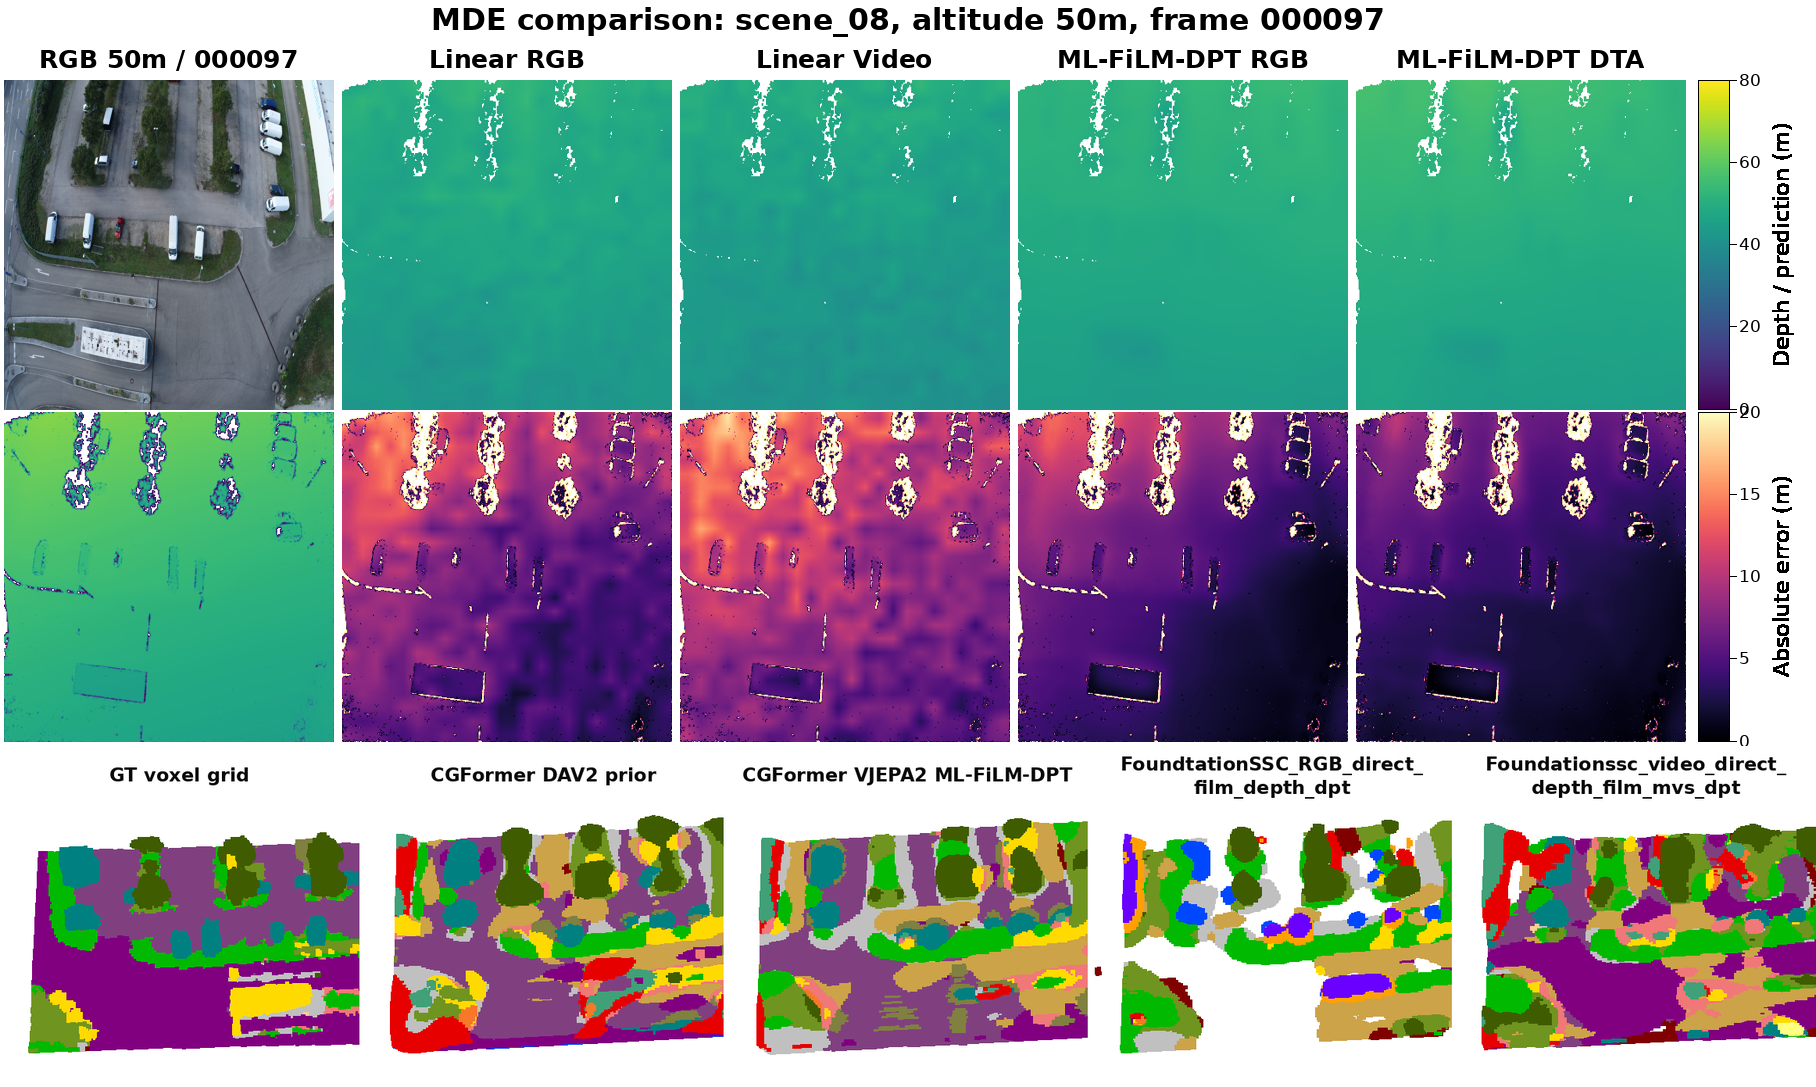
\includegraphics[width=0.98\linewidth]{content/images/ssc/scene_08_50_000097_mde_appended_ssc.png}
\caption{Qualitative OccuFly depth and SSC example for scene 08 at 50~m altitude, frame 000097.}
\label{fig:occufly_ssc_qualitative_scene_08_50_000097}
\end{figure}

\FloatBarrier
